%===============================================================
\section{Background}
\setcounter{section}{1}

%===============================================================
% Background on Browsers
%===============================================================
\subsection{Browsers}
In the thirty years since \textit{WorldWideWeb}\cite{berners-lee_www}, the first web browser,
the architecture of the \textsc{World Wide Web (Web)}, and thus web browsers, has exponentionally grown
in both complexity and use. Global strives in consumer technology have allowed billions\cite{browser-stats-world} of users to
access the \textsc{Web}, often through a web browser. Naturally static HTML pages were insufficient;
users wanted \textit{interactive} pages, custom page styling, support for additional media types,
and interconnectivity between two or more \textsc{Web} resources. Today, the \textsc{Web} still
uses HTML, but it's architectural tours de force is the JavaScript language\protect\footnotemark.
\footnotetext{Amoung numerous others, e.g.: PHP, WASM, Go-lang, CSS, etc.}%

\noindent
Modern browsers are built on layed components, running at least two processes: (1) A
primary (main) browser process, for the application itself, and (2) one or more renderer
process. An example architectual diagram is provided as \textit{Figure 1}.%
% Browser Components %
\begin{figure}[!h]
    \begin{center}
        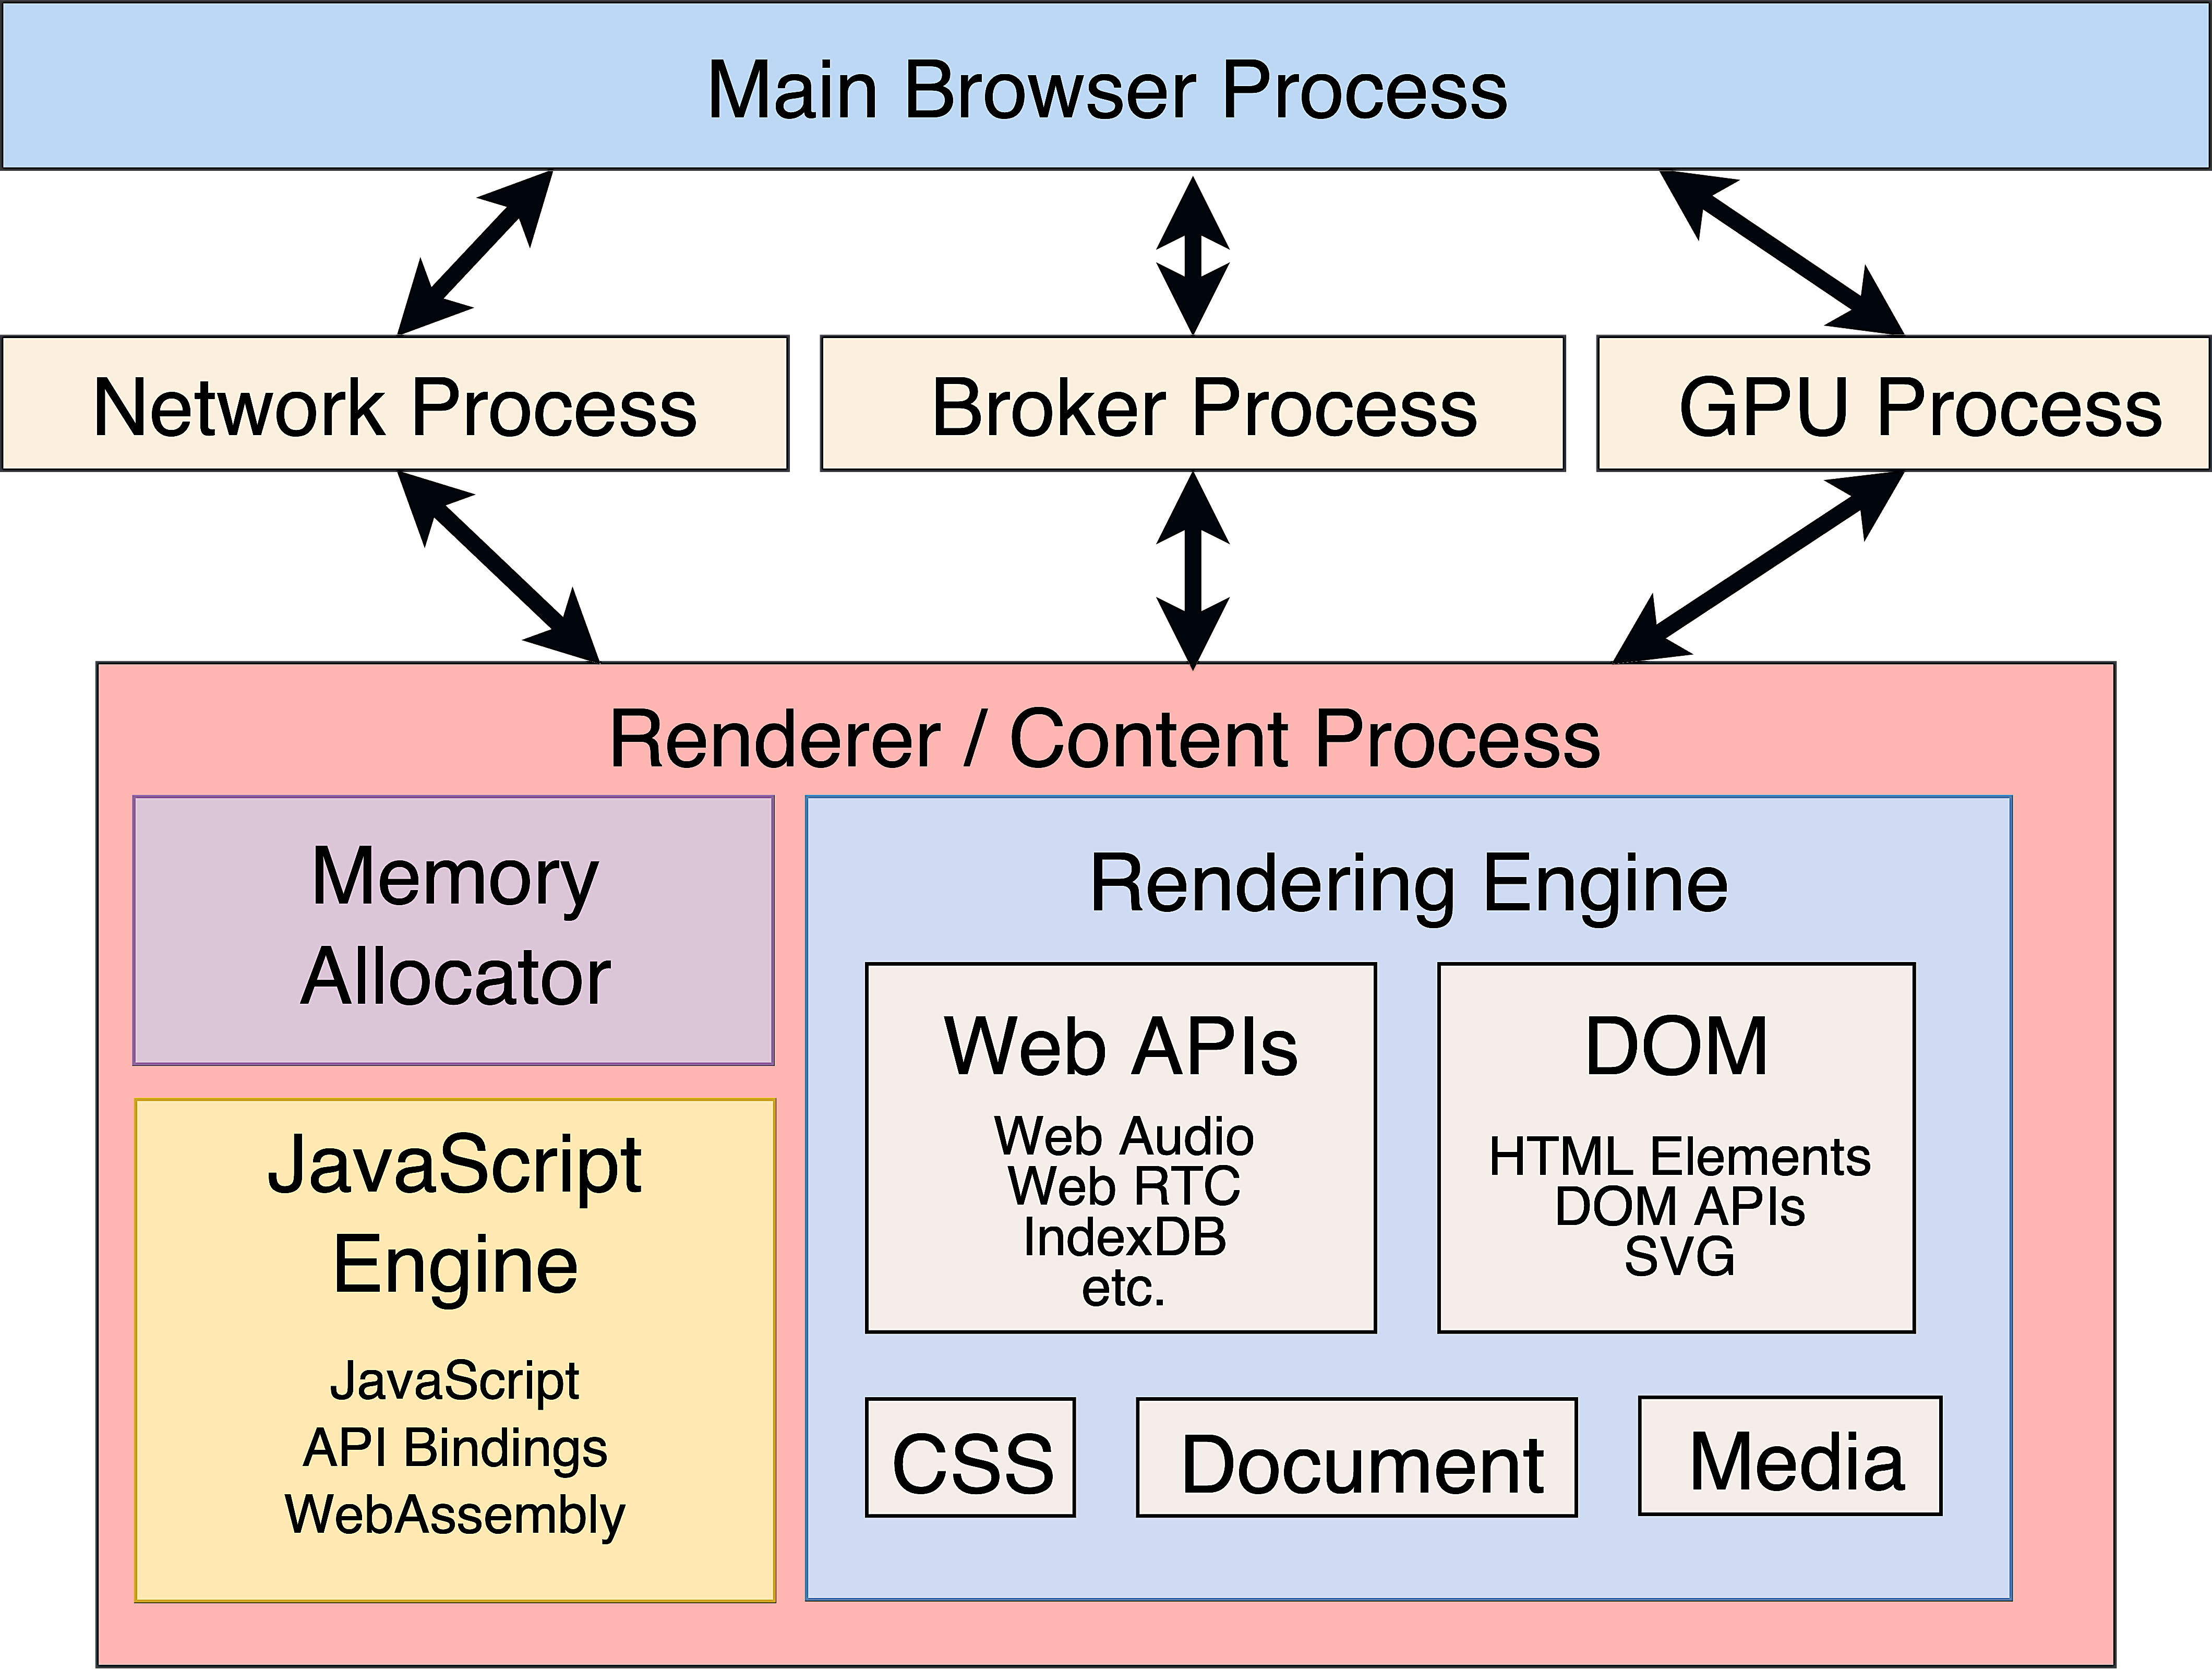
\includegraphics[width=0.475\textwidth]{./img/browser-process-architecture}
        \caption{Process achitecture of a modern web browser.}
    \end{center}
    \vspace{-4ex}
\end{figure}

%% Definition: \newcommand{\p}[1]{\paragraph{\itseries\scshape{#1}}}
\p{Main Browser Process }%
This process is the primary controller for all computaiton; it displays the user interaface and
manages the all processes. Safari, specifically, utilizes a split-process model\cite{wk2}, where
each tab's web content lives in a seperate, isolated, renderer (web) process, spawned per tab.
Although this model improves stability and performance, it's greatest significance is this model
also provides the basis for a sandboxing infrastructure; ideally one that will limit damage
to the system, if a rederer process is compromised.

\p{Renderer Process. }%
This component parses \textsc{HTML}, \textsc{CSS}, \textsc{JS}, numerous image/video formats,
and any other varing data formats required to construct the document.
In additional to the core language features, numerous browser APIs allow
developers to interact with this document, or rather Document Object Model
(DOM), retreive data over the network, access web databases, and
more $-$  all via JavaScript. \\
% WebKit Component Boundaries %
% TODO: Remove this if no longer needed
%\begin{figure}
%    \begin{center}
%        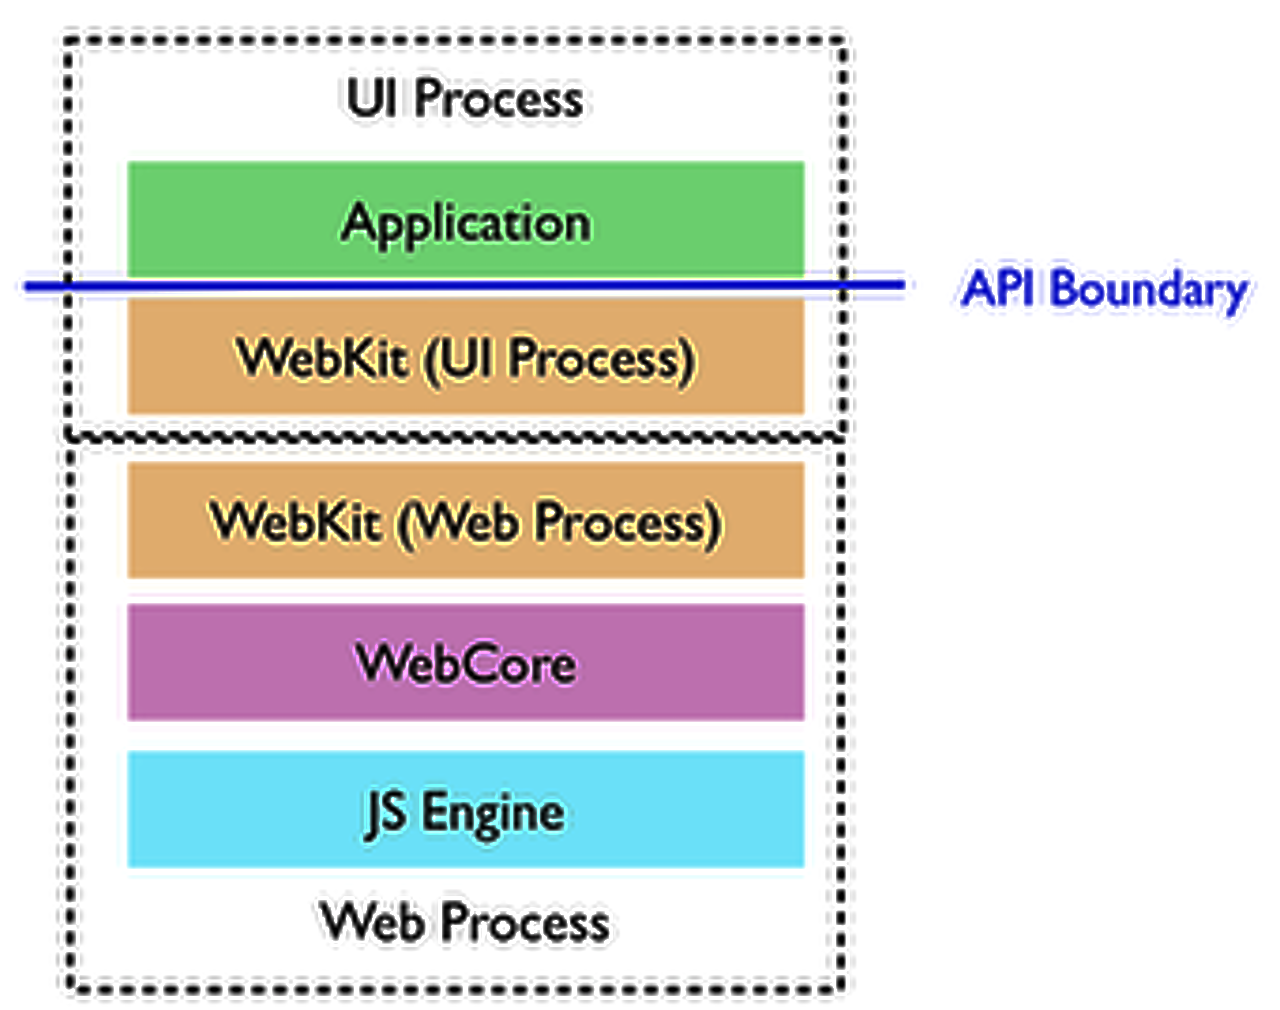
\includegraphics[width=0.475\textwidth]{img/inv}
%    \end{center}
%    \caption{WebKit Process Model}\vspace{-5ex}
%\end{figure}

From a security standpoint, the renderer retreives, lexes, parses, compiles [to C++], and
displays a multitude of untrusted and potentially complex JavaScript inputs; it is the most
exposed browser component. As such, it's commonly sandboxed\protect\footnotemark, limiting
access to sensitive data and applications, both internally and within the device's operating
system or underlying kernel.
\footnotetext{The complements of this paper's work can found here <link to zach's paper/stuff>}

%===============================================================
% Background on JS engines and JavsScriptCore
%===============================================================
\subsection{JavaScript Engines}
JavaScript, a weakly-typed scripting language, is one of the largest components of modern websites.
Naturally, the need for high performance script exectuion resulted in deeply complex engine
implementations; the perfect place to hunt for complex, domain-specific vulnerabilities. Modern
JavaScript engine typically consist of a runtime and the following components:

\p{Parser and Bytecode Compiler. }%
The parser and bytecode compiler are responsible for converting JavaScript source
code to an engine-specific bytecode representation, for use by the interpreter and JIT
compiler. Parsing tokenizes the input stream and contructs an Abstract Syntax Tree (AST)
based on grammartical sytax of JavaScript. The AST is subsequently compiled to bytecode.%
%(i) a parser and bytecode compiler, (ii) an interpreter for aforementioned bytecode,
%(iii) at least one Just-in-Time (JIT) compiler, (iv) and a memory allocation mamangement system, a Garbage Collector (GC).
%
%
% integrate bytecode example better %
\begin{lstfloat}
\begin{lstlisting}[style=JS,caption=Example function to JIT compiler]
// add.js
function add(a,b) {
    return a + b;
}
add(2, 1337);
\end{lstlisting}
\end{lstfloat}
%
\vspace{-1.5em}\noindent
The bytecode is the source of truth throughout the whole engine. While some engines, such as
Spidermonkey, use a stack-based virtual machine, other engines, e.g., JavaScriptCore, use a register-based
virtual machine. As such, their bytecode format is fundamentally different. However, one typically common
shared property is that bytecode is untyped: the bytecode operates on weakly-typed values which
contain both type- and value-information. During execution, an interpreter will perform
different actions depending on the runtime type of the operands.
%
\begin{lstfloat}
\begin{lstlisting}[style=asm, caption=Interpreter bytecode and type profile]
// jsc -d add.js
bb#1
[   0] enter
[   1] get_scope    dst:loc4
[   3] mov          dst:loc5, src:loc4
[   6] check_traps
[   7] add          dst:loc6, lhs:arg1, rhs:arg2, operandTypes:OperandTypes(126, 126)
[  13] ret          value:loc6
\end{lstlisting}
\end{lstfloat}
%
\vspace{-1.5em}\noindent
Another property common to the resulting bytecode is that it is usually unoptimized. This is primarily done
for two reason: (1) To keep the overall startup time as low as possible, forbidding the use of costly
optimizations, and (2) many optimizations require type information, which is not available at this point,
due to the weakly-typed nature of the language itself.
%
\p{Interpreter. }%
The task of an interpreter is to consume the bytecode and execute it. As the bytecode is specific to
a given engine, so id the interpreter. Interpretation happens by fetching the next bytecode instruction
from the currently executing code and dispatching it to the handler for the bytecode operation.

\noindent
While interpretation of bytecode is fairly slow, in part due to the unoptimized nature of the bytecode
and high dispatching overhead, the initial startup time is minimal. Thus, for simple or sparsly repeated
operations it's overall better to execute it directly via the interpreter; the overhead compilation
would introduce simply outweighs the faster execution speed of the resulting machine code. Conversely,
if code segment/block is repeatedly executed by the application it is worth optimizing that code. This is
the job of a JIT compiler. As current JIT compilers usually require type hints to produce optimized machine
code, it's also the job of the interpreter to collect type profiles during bytecode execution. Often this
is performed by augmenting the bytecode with previously seen input types for each bytecode operation. An
example of bytecode after it has gone through this process in JavaScript core is provided in 
\textit{Listing 3}, below.
% JSC takes this even further, 'typed' bytecode is interpretted and used to perform speculative optimization %
% (^) footnote or section? %

%===============================================================
% JSC Bytecode interpreter
% JSC specifics on bytecode and register typing %
%   Not sure where to put this, yet - if at all %
%With the new infrastructure, when declaring an instruction, a name and type must be given for each
%of the operands, as well as declaring all the data that will be stored in the metadata table.
%
\begin{lstfloat}
\begin{lstlisting}[style=JS,caption=JavScriptCore SyntaxType for OpAdd]
op:add,
  args: {
    dst: VirtualRegister,
    lhs: VirtualRegister,
    rhs: VirtualRegister,
    operandTypes: OperandTypes,
  },
  metadata: {
    arithProfile: ArithProfile,
  }
\end{lstlisting}
\end{lstfloat}%
\vspace{-2.5em}%
%With this extra information, it is now possible to generate a fully typed struct for each instruction:
%
%\begin{lstfloat}
%\begin{lstlisting}[style=JSC++,caption=JavScriptCore Syntax Type for OpAdd]
%SLOW_PATH_DECL(slow_path_add)
%{
%   OpAdd bytecode = pc->as<OpAdd>();
%   JSValue lhs = GET_C(bytecode.m_lhs);
%   JSValue rhs = GET_C(bytecode.m_rhs);
%   ...
%}
%\end{lstlisting}
%\end{lstfloat}
%
%In the example above, we first need to convert the generic \textsc{Instruction* pc} to the instruction we
%want to access, which will perform a runtime check. If the opcode matches, it returns an instance
%of the generated struct, OpAdd, which includes the fields \textbf{m\_lhs} and \textbf{m\_rhs}, both of type VirtualRegister as specified in our instruction declaration.
%===============================================================
%
%
\p{JIT Compiler. }%
A JIT compiler acts as an alternative to an interpreter for script execution. It, too,
consumes bytecode by the parser, as well as type profiles gathered during execution by the
interpreter.  Having access to both, it converts the bytecode to optimized machine code which
can be executed directly on the host CPU.%

\noindent
As JIT compilers are crucial to execution performance, they are the subject of intensive research.
Many implementations and key mechanisms have been discussed, e.g., polymorphic inline
caches\protect\footnotemark.
\footnotetext{Polymorphic Inline Caching is a broadly used mechanism to speed up polymorphic
operations in dynamic language interpreters and at the same time gather type information
for the JIT compiler by caching results of previous executions.}

\noindent
A JIT compiler will often, initially, convert the bytecode to another custom intermediate representation.
This IR is often graph based to facilitate the various optimizations that are later performed on it. In
addition, most engines currently use a static single assignment (SSA) form to further simplify code
analysis and optimization; JavaScriptCore utilizes a two-tier IR consisting of Bare Bones IR and AIR.%
% code snip examples? %

\subparagraph{\textit{Speculative Optimization. }}%
% we focus on the JIT compilers: DFG,FTL
% go through DFG vuln example
One essential mechanism that allows generation of performant machine code for JavaScript
and dynamically typed languages, in general, is speculations: equipped with type profiles from the
interpreter, the compiler \textit{speculates} that the same types will be used in the future. It will
then guard these assumptions with runtime guards: small fragments of code that perform an inexpensive
type check and bailout if the check fails, in which case execution will continue in a more generic
execution tier, i.e., the interpreter. These type-guards essentially convert the previously untyped
code into strictly typed code, which may subsequently be optimized in a similar fashion as other
strictly-typed languages, such as C++ or Java. This mechanism is shown in \textit{Listing 4} using an
imaginary bytecode and compiler IR format.

\begin{lstfloat}
\begin{lstlisting}[style=JS,caption=Compiler IR for interpreter bytecode\protect\footnotemark]
function add:
  v0 = LoadArgument 0  
  CheckIsInteger v0

  v1 = LoadArgument 1  
  CheckIsInteger v1
    
  v2 = IntegerAdd v0, v1
  Return v2
\end{lstlisting}
\end{lstfloat}
\footnotetext{Type profiles were used to emit type checks and optimiatize specialized integer addition instructions.}

\vspace{-1.5em}\noindent
It is not uncommon for an engine to have multiple levels of JIT compilers.  These correspond to
different optimization levels: the early JIT compilers perform less optimizations, thereby produce
machine code faster. The late JIT compiler stages perform more optimizations,thereby generating
faster machine code.  A unit of code may be recompiled by a higher level JIT compiler when its
execution count reaches another threshold.  JavaScriptCore, the engine inside WebKit currently
features three different JIT compilers in addition to an interpreter. V8, the engine inside the
Chrome browser, on the other hand, only uses one JIT compiler and one interpreter.%

\begin{figure*}[!t]
\begin{center}
    \vspace{-5em}
    \begin{minipage}{\dimexpr\paperwidth}
    %\def\svgwidth{584bp}
    \def\svgwidth{\paperwidth}
    \scalebox{0.85}{\input{./img/optimization-workflow-c-vs-js.pdf_tex}}\vspace{-2em}
    \end{minipage}
\end{center}
\caption{JSC Speculative Optimization WorkFlow}
\end{figure*}

\noindent
Here, the function to be compiled, which is shown in \textit{Listing 1} is invoked with integers as arguments. This is
captured by the interpreter in-type profiles associated with the bytecode as shown in \textit{Listing 2}.
Based on those, the JIT compiler speculates that the same types will be used in the future and guards
that assumption with two type checks. Afterwards, the compiler can use fast, specific operations, such
as the addition of two integers, in lieu of slow, generic ones that cover all possible scenarios of
different types. This can be seen in \textit{Listing 3}. The integer addition used in this example could well
be implemented with a single machine instruction instead of the generic addition operation as defined
by the language specification.%
% TODO: Add img/ftl_pipeline.png somewhere %

\p{Garbage Collection. }%
As JavaScript frees the programmer of the responsibility to return allocated memory back
to the system, it requires a garbage collector (GC) to detect and reclaim unused memory.%

\noindent
Most high-performance garbage collector systems are based on the mark-and-sweep algorithm, which
operates in two phases. First, during the periodic marking phases, the whole graph of reachable
objects is scanned. Then, during the sweeping phase, every memory allocation which was not visited,
implying that it is a dead object, is freed and returned to the allocator.%

\noindent
Various extensions of this core algorithm exist and are in use today. One key improvement lies
in concurrent marking to avoid noticeable pauses in the application caused by ”stop-the-world”
garbage collection. Modern collectors such as \textsc{Riptide}\protect\footnotemark, the collector used in
JavaScriptCore, further strive for a minimal amount of application interrupts due to garbage
collection through parallelism, if multiple CPU cores are available.
\footnotetext{\textsc{Riptide}, was not targeted for this research.}

%===============================================================
